\documentclass[nobib]{tufte-handout}


\usepackage{ifluatex, ifxetex} % проверка, как компилируется файл

% black magic!
% solving problem with tufte-handout + xelatex
% http://tex.stackexchange.com/questions/200722/
% https://tex.stackexchange.com/questions/47576/
\ifx\ifxetex\ifluatex\else % если xelatex или lualatex
  \newcommand{\textls}[2][5]{%
    \begingroup\addfontfeatures{LetterSpace=#1}#2\endgroup
  }
  \renewcommand{\allcapsspacing}[1]{\textls[15]{#1}}
  \renewcommand{\smallcapsspacing}[1]{\textls[10]{#1}}
  \renewcommand{\allcaps}[1]{\textls[15]{\MakeTextUppercase{#1}}}
  \renewcommand{\smallcaps}[1]{\smallcapsspacing{\scshape\MakeTextLowercase{#1}}}
  \renewcommand{\textsc}[1]{\smallcapsspacing{\textsmallcaps{#1}}}
\fi

% с альтернативного источника:
%\ifluatex % Allow rendering with LuaTeX by setting up the spacing using fontspec features
%  \renewcommand\allcapsspacing[1]{{\addfontfeature{LetterSpace=15}#1}}
%  \renewcommand\smallcapsspacing[1]{{\addfontfeature{LetterSpace=10}#1}}
%\fi

% lua produces strange notes
% https://tex.stackexchange.com/questions/328431

\usepackage{fontspec} % работа со шрифтами
%\usepackage{polyglossia} % учим русский как иностранный :)

%\setmainlanguage{engish}
%\setotherlanguages{english}

% заменяем --- на тире, << на кавычки и т.д.:
\defaultfontfeatures{Ligatures=TeX}

% download "Linux Libertine" fonts:
% http://www.linuxlibertine.org/index.php?id=91&L=1
\setmainfont{Linux Libertine O} % or Helvetica, Arial, Cambria
% why do we need \newfontfamily:
% http://tex.stackexchange.com/questions/91507/
\newfontfamily{\cyrillicfonttt}{Linux Libertine O}
\newfontfamily{\cyrillicfont}{Linux Libertine O}
\newfontfamily{\cyrillicfontsf}{Linux Libertine O}



\usepackage{amsmath}
\usepackage{amsthm}
\usepackage{amsfonts}
\usepackage{amssymb}
\usepackage{url} % вставка \url{}
\usepackage{graphicx} % вставка графиков
\usepackage{csquotes} % адаптирующиеся кавычки командой \enquote{}
\usepackage{comment} % ingore everything between \begin{comment} \end{comment}
\usepackage{answers} % separate problems and solutions
\usepackage{tikz} % pictures with tikz language
\usepackage{todonotes} % todo in documents
\usepackage{multicol} % make several columns
\usepackage{subfigure}

\usepackage{enumitem} % для создания своих нумерующих списков (хак для гиперссылок)

%\usepackage[left=2cm,right=2cm,top=2cm,bottom=2cm]{geometry}


% very useful during de-bugging!
% \usepackage[left]{showlabels}
% \showlabels{hypertarget}
% \showlabels{hyperlink}


\DeclareMathOperator{\Var}{Var}
\DeclareMathOperator{\sVar}{sVar}
\DeclareMathOperator{\pVar}{pVar}
\DeclareMathOperator{\card}{card}
\DeclareMathOperator{\Cov}{Cov}
\DeclareMathOperator{\Corr}{Corr}
\DeclareMathOperator{\sCov}{sCov}
\DeclareMathOperator{\pCov}{pCov}
\DeclareMathOperator{\sCorr}{sCorr}
\DeclareMathOperator{\pCorr}{pCorr}
\DeclareMathOperator{\E}{E}
\renewcommand{\P}{\mathbb{P}}
\newcommand{\I}{\mathbb{I}} % индикатор события
\newtheorem{theorem}{Theorem}
\newtheorem{corollary}{Corollary}[theorem]
\newtheorem{lemma}[theorem]{Lemma}
\theoremstyle{definition}
\newtheorem{definition}{Definition}

\usepackage[bibencoding = auto, backend = biber,
sorting = none]{biblatex}

%\addbibresource{probability_dna.bib}



%\title{Geometric interpretaion of main concepts and theorems in econometrics}
\title{some title}
\author{}
\date{\today}
\begin{document}

\maketitle

%\section{Literature review}

\section{Regression}

\subsection{Sample correlation}

\marginnote{
\begin{align*}
\sCorr(x,y) &= \frac{\sCov(x,y)}{\sqrt{\sVar(x)\sVar(y)}} \\
&= \frac{\frac{1}{n-1}\sum_{i=1}^n (x_i - \bar x)(y_i - \bar y)}{\sqrt{\frac{1}{n-1} \sum_{i=1}^n (y_i - \bar y)\frac{1}{n-1} \sum_{i=1}^n (\hat y_i - \bar{\hat y})}}
\end{align*}
}

The most crucial part in defining correlation geometrically is definig the dot product as it enables to compute the length of a vecotr:
\[
|\vec{a}| = \sqrt{\langle \vec{a},  \vec{a}\rangle}
\]
and the angle between any two vectors:
\[
\cos(\vec{a}, \vec{b}) = \frac{\langle \vec{a},  \vec{a}\rangle}{|\vec{a}| |\vec{b}|}
\]
Now we define scalar product of two vectors
$x =
\begin{pmatrix}
x_1 \\
\vdots \\
x_n
\end{pmatrix}$
and
$y =
\begin{pmatrix}
y_1 \\
\vdots \\
y_n
\end{pmatrix}$
as a sample covariation between them:
\[
\langle x, y \rangle = \sCov(x, y)
\]
The main characteristics of a vector are its length and direction.
So, we introduce the length
\[
\sqrt{\sCov(x,x)} = \sqrt{\sVar(x)} = \sigma_x
\]
and the angle between two random vectors
\[
\cos(x,y) = \frac{\sCov(x,y)}{\sqrt{\sVar(x)\sVar(y)}} = \sCorr(x,y)
\]
Note that from the definition of the angle it follows that the sample correlation can range from $-1$ to $1$.

\begin{figure}[h!]
\begin{center}
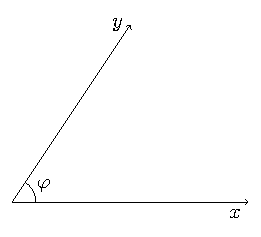
\includegraphics[width=0.4\linewidth]{images/corr_def.pdf}
\caption{Vector $x$ of length $\sigma_x$ and random vector $y$ of length $\sigma_y$, $\cos \varphi$ is the angle between $x$ and $y$.}
\label{fig:corr_def}
\end{center}
\end{figure}

Another important geometrical tool is projection. Recall that for any two vectors the scalar product $\langle \vec{a}, \vec{b} \rangle$ can be interpreted as the length of projected $\vec{b}$ multuplied by the length of $\vec{a}$.
The projection itself is $cos(\vec{a}, \vec{b}) \vec{b}$.
Same holds for the vectors sampled from some distribution.
The projection of such a vector $y$ onto $\{cx| c \in \mathbb{R}\}$ is $\hat y = \sCorr(x,y) \cdot y$.

\begin{figure}[h!]
\begin{center}
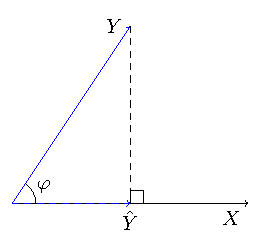
\includegraphics[width=0.4\linewidth]{images/corr_proj.pdf}
\caption{Vector $y$ projected onto vector $x$.}
\label{fig:corr_proj}
\end{center}
\end{figure}

Looking at Figure~\ref{fig:corr_proj}, we can interpret the square of sample correlation coefficient.
Using the fact that $cos^2 \varphi$ is the squared ratio of the leg adjacent to $\varphi$ to hypotenuse, we can conclude that
\[
\sCorr^2(x,y) = \frac{\sVar(\hat y)}{\sVar(y)}
\]
as the variance of a vector is associated with the square of its length.
Thus, the sample correlation coefficient squared shows the fraction of variance in $y$ which can be explained
with the most similar vector proportional to $x$.


\subsection{Sample correlation when a constatnt vector added}

\marginnote{
\begin{align*}
\sCorr(x + \alpha \mathbf{1}, y) &= \frac{\sCov(x + \alpha \mathbf{1}, y)}{\sVar(x + \alpha \mathbf{1}) \sVar(y)} \\
&= \frac{\sCov(x,y)\sCov(\alpha \mathbf{1},y)}{\sVar(x)\sVar(y)} \\
&= \frac{\sCov(x,y)}{\sVar(x)\sVar(y)} \\
&= \sCorr(x,y)
\end{align*}
}

\begin{theorem}
Adding a vector of constants does not affect the sample correlation coefficient:
\[
\sCorr(x + \alpha \mathbf{1}, y) = \sCorr(x,y)
\]
where $\alpha \in \mathbb{R}$.
\end{theorem}

\begin{proof}
Firstly, we project vectors $x$ and $y$ onto $Lin^{\perp}(\mathbf{1})$ in order to get $x^c = x - \bar x$ and $y^c = y - \bar y$
(`c' stands for `centred'). It can be shown that the matrix corresponding to projecting onto the line spanned by a vector of all ones has the following form
\[
\frac{\mathbf{1}^T \mathbf{1}}{\mathbf{1} \mathbf{1}^T} = \frac{\begin{pmatrix} 1 & \ldots & 1 \end{pmatrix} \begin{pmatrix} 1 \\ \vdots \\ 1 \end{pmatrix}}{\sum_{i=1}^n 1} = \begin{pmatrix} \frac{1}{n} & \ldots & \frac{1}{n} \\ \vdots & \ddots & \vdots \\ \frac{1}{n} & \ldots & \frac{1}{n} \end{pmatrix}
\]
Thus, projecting onto an orthogonal subspace is equivalent to substracting the projected vector, i.e., the vector of averages, from the original one.

Also note that the angle $\varphi$ between original and centred vectors remains the same.
The results of this step is shown in Figure~\ref{fig:corr_xyc}.

\begin{figure}[h!]
  \centering
  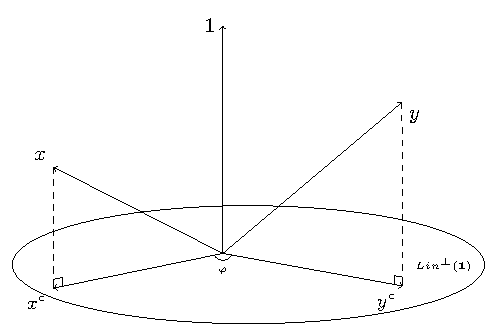
\includegraphics[width=0.45\linewidth]{images/corr_const_cent.pdf}
  \caption{Centred vectors $x^c$ and $y^c$}
  \label{fig:corr_xyc}
\end{figure}

Then we need to derive a new vector $\tilde x$ with constants added to each component.
Geometrically adding a vector of costants means adding a vector of all ones
scaled by $\alpha \in \mathbb{R}$, i.e., $\alpha \mathbf{1}$.
Then the new vector $\tilde x$ can be broken up into a sum of $\alpha \mathbf{1}$ and
$\beta x$, $\alpha, \beta \in \mathbb{R}$, which can be seen in Figure~\ref{fig:corr_tildex}.
After that we will project this new vector $\tilde x$ onto $Lin^{\perp}(\mathbf{1})$.
By the properties of projection it is of no difference whether to project
the whole vector $\tilde x$ or project its parts $\alpha \mathbf{1}$
and $\beta x$ — the result is the same.
So, while $\beta x$ is projected onto a span of $x^c$, the projection of $\alpha \mathbf{1}$
onto the orthohgonal space $Lin^{\perp}(\mathbf{1})$ yields zero as demonstrated
in Figure~\ref{fig:corr_tildex}.
Moreover, it follows that the angle between $\tilde x$ and $y$ is still $\varphi$.

\begin{figure}
  \centering
  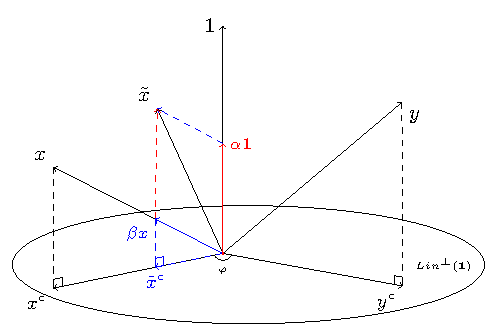
\includegraphics{images/corr_const_br_up.pdf}
  \caption{Decomposition and projection of $\tilde x$}
  \label{fig:corr_tildex}
\end{figure}

Finally, putting everything together we finish the proof:
\[
\sCorr(x + \alpha \mathbf{1}, y) = \sCorr(x,y)
\]

\begin{figure}
  \centering
  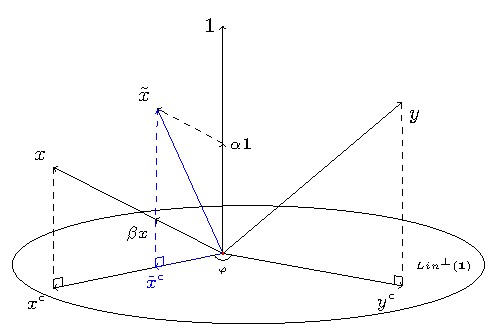
\includegraphics{images/corr_const_final.pdf}
  \caption{$\sCorr(x + \alpha \mathbf{1}, y) = \sCorr(x,y)$ as the corresponding angles are equal.}
  \label{fig:corr_final}
\end{figure}


\end{proof}

\subsection{Sample correlation coefficient in simple linear regression}

\marginnote{
Assuming the underlying relationship between $x$ and $y$ to be
\[
y_i = \beta_1 + \beta_2 x_i + \varepsilon_i \quad i=1,\ldots,n
\]
where $\varepsilon_i$ is an error term the following holds
\begin{align*}
\sCorr(y, \hat y) &= \frac{\sCov(y)\sCov(\hat y)}{\sqrt{\sVar(y)\sVar(\hat y)}} \\
&= \frac{\sCov(y)\sCov(\hat \beta_1 + \hat \beta_2 x)}{\sqrt{\sVar(y)\sVar(\hat \beta_1 + \hat \beta_2 x)}} \\
&= \frac{\sCov(y)\sCov(\hat \beta_2 x)}{\sqrt{\sVar(y)\sVar(\hat \beta_2 x)}} \\
&= \frac{\hat \beta_2 \sCov(y)\sCov(x)}{|\hat \beta_2| \sqrt{\sVar(y)\sVar(x)}} \\
&= sign(\hat \beta_2) \frac{\sCov(y)\sCov(x)}{\sqrt{\sVar(y)\sVar(x)}}
\end{align*}
}

\begin{theorem}
A linear regression model with one explanatory variable and constant term
\[
y = \beta_1 + \beta_2 x + \varepsilon
\]
has the property
\[
\sCorr(y, \hat y) = sign(\hat \beta_2) \sCorr(y, x)
\]
\end{theorem}

\begin{proof}
Firstly, we consider the case when $\hat \beta_2 > 0$ so the main picuture is of the form depicted in Figure~\ref{fig:corr_pos_base}.
It has been shown earlier that the correlation coefficient represents the angle betweem two random vectors.
So in order to complete the proof we need to find the appropriate angles and compare them.

\begin{figure}[h!]
\center{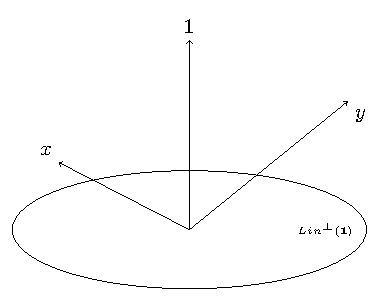
\includegraphics[width=0.35\linewidth]{images/corr_eq_positive.pdf}}
\caption{Vectors $x$, $y$ and $\mathbf{1}$.}
\label{fig:corr_pos_base}
\end{figure}

However, it seems to be difficult to compare the angles in the three dimensional space.
That is why we start with projecting both $x$ and $y$ onto the space perpendicular to the vector of all ones $\mathbf{1}$ as shown in Figure~\ref{fig:corr_pos_xyc}.
We denote this space as $Lin^{\perp}(\mathbf{1})$. The resulting vectors are $x - \bar x \cdot \mathbf{1}$  and $y - \bar y \cdot \mathbf{1}$ respectively
since projection of any vector $\vec{a}$ on the line given by a vector of all ones yields the vector of averages $\vec{\bar a}$.

In order to get the angle between $y$ and $\hat y$ we should start with regressing $y$ on $Lin(x, \mathbf{1})$.
Then the only thing thing left is to project $\hat y$ onto $Lin^{\perp}\mathbf{1}$ since the $y$ vector has already been projected.
Note that the projected $\hat y$ falls onto tha span of vector $x - \bar x \cdot \mathbf{1}$ as it can be decomposed into a sum $a x + b \mathbf{1}$ where $a, b \in \mathbb{R}$.
$a x$ is projected in the same way as $x$ and $b \mathbf{1}$ yields zero when projected onto the orthogonal space.
The result of this step is shown in Figure~\ref{fig:corr_pos_yhatc}.

\begin{figure}[h!]
\begin{center}
\subfigure[]{
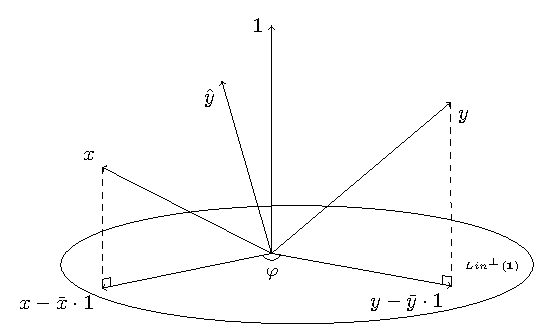
\includegraphics[width=0.6\linewidth]{images/corr_eq_positive_xy_centered.pdf}
\label{fig:corr_pos_xyc}}
%\hspace{4ex}
\subfigure[]{
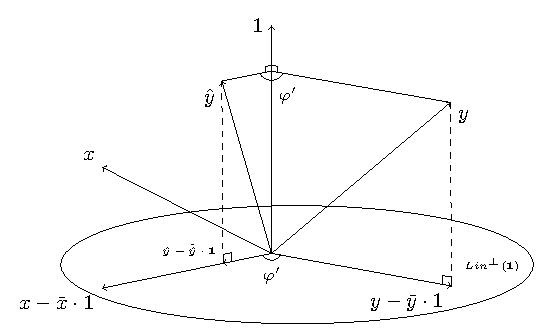
\includegraphics[width=0.6\linewidth]{images/corr_eq_positive_yhat.pdf}
\label{fig:corr_pos_yhatc}}
\caption{\subref{fig:corr_pos_xyc}: `Centred' $x$ and $y$, i.e., projected onto $Lin^{\perp}(\mathbf{1})$; \subref{fig:corr_pos_yhatc}: `Centred' $\hat y$, i.e., projected onto $Lin^{\perp}(\mathbf{1})$.}
\end{center}
\end{figure}

Since the projection of $\hat y$ lies exactly on the span of vector $x - \bar x \cdot \mathbf{1}$, we can conclude that $cos \varphi = \cos \varphi '$ and to put it another way $\sCorr(x,y) = \sCorr(y, \hat y)$.

Now consider the case when $\hat \beta_2 < 0$.
Note that the sign of $\beta_1$ does not influence the correlation coefficient sign.
The only difference is that now $\hat y$ is projected onto the span of  $x - \bar x \cdot \mathbf{1}$ and not on this vector itself while the projections of $x$ and $y$ remain the same.
Looking at Figure~\ref{fig:corr_negative} we deduce that the angle betwween $y$ and $\hat y$ is compelement to the angle between $x$ and $y$.
Using trigonometric properties, we simplify $\cos(180^{\circ} - \varphi) = -\cos\varphi$ which in turn implies $\sCorr(x,y) = -\sCorr(y,\hat y)$.

\begin{figure}[h!]
\begin{center}
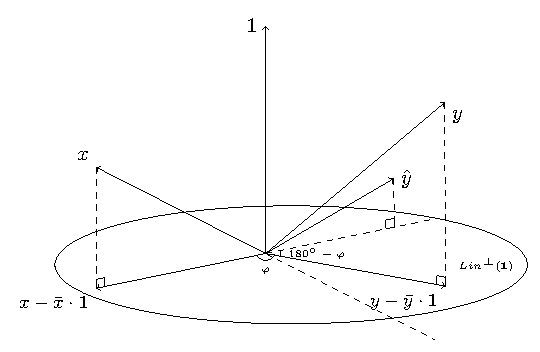
\includegraphics{images/corr_eq_negative.pdf}
\label{fig:corr_negative}
\caption{Case of $\beta_2 < 0$.}
\end{center}
\end{figure}
\end{proof}


\subsection{RSS + ESS = TSS}

\marginnote{
Consider a regresion model with $n$ observations and $k$ explanatory variables including a constant unit vector
\[
y = X \beta + \varepsilon
\]
The OLS estimator for the vector of coefficients $\beta$ is
\[
\hat \beta = (X^T X)^{-1} X^T y
\]
and the residual vector is
\begin{align*}
\hat e &= y - \hat y \\
&= y - X \hat \beta \\
&= y - X (X^T X)^{-1} X^T y
\end{align*}
Then we define residual sum of squares (RSS), explained sum of squares (ESS) and total sum of squares (TSS) as follows:
\begin{align*}
RSS &= \lVert y - \hat y \rVert^2_2 \\
ESS &= \lVert \hat y - \bar y \rVert^2_2 \\
TSS &= \lVert y - \bar y \rVert \\
\end{align*}
Disclosing parentheses and using the fact that $\hat{y}^T y = \hat{y}^T \hat{y}$
\begin{align*}
\hat{y}^T y &= \beta^T X^T y \\
&=  y^T X (X^T X)^{-1} X^T y \\
\hat{y}^T \hat{y} &= \beta^T X^T X \beta \\
&= y^T X (X^T X)^{-1} X^T X (X^T X)^{-1} X^T y \\
&= y^T X (X^T X)^{-1} X^T y
\end{align*}
we obtain
\begin{align*}
RSS &= y^T y -\hat{y}^T \hat{y} \\
ESS &= \hat{y}^T \hat{y} - \hat{y}^T \bar{y} + \bar{y}^T \bar{y} \\
TSS &= y^T y - 2 y^T \bar y +  \bar{y}^T \bar{y}
\end{align*}
When putting everything together all the terms cancel out which proves
\[
ESS + RSS = TSS
\]
}

\begin{theorem}
A linear regression model with $n$ observations and $k$ explanatory variables including a constant unit vector
\[
y = X \beta + \varepsilon
\]
has the following property
\[
RSS + ESS = TSS
\]
where $RSS = \lVert y - \hat y \rVert^2_2$, $ESS = \lVert \hat y - \bar y \rVert^2_2$, $TSS = \lVert y - \bar y \rVert^2_2$.
\end{theorem}

\begin{proof}
The proof will be presented for the case of two regressor $x$ and $\mathbf{1}$ in order for the picture to be clear.
However, the same logic applies for the case of $k$ regressors.

We start with depicting the vectors $y \in \mathbb{R}^{n-2}$ and $x, \mathbf{1} \in \mathbb{R}^2$.
Then we project $y$ onto $Lin(x, \mathbf{1})$ and obtain $\hat y$ which is shown in Figure~\ref{fig:tss_base}.

From this picture we can immediately derive $\sqrt{RSS}$ as by definition this is the squared difference between $y$ and $\hat y$.

\begin{figure}[h!]
\begin{center}
\subfigure[]{
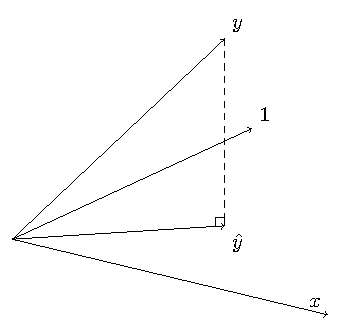
\includegraphics[width=0.4\linewidth]{images/tss_sum_base.pdf}
\label{fig:tss_base} }
\hspace{4ex}
\subfigure[]{
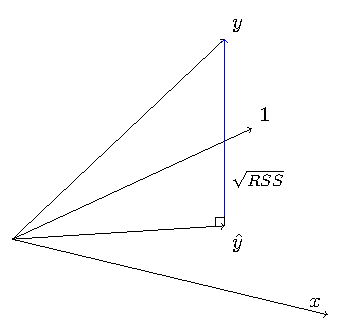
\includegraphics[width=0.4\linewidth]{images/tss_sum_rss.pdf}
\label{fig:tss_rss}}
\caption{\subref{fig:tss_base}: Vectors $y \in \mathbb{R}^{n-2}$ and $\hat y \in Lin(x, \mathbf{1})$; \subref{fig:tss_rss}: Residual sum of squares.}
\end{center}
\end{figure}

So as to visualize $ESS$ and $TSS$ we first need to visualize vector of averages $\bar y$.
Geometrically this means projecting a vector onto a line spanned by vector $\mathbf{1}$.

Now we both project $y$ and $\hat y$ onto $\mathbf{1}$ and following the definition obtain $\sqrt{TSS}$ as the difference vector $y - \bar y$ and $\sqrt{ESS}$ as the vector $\hat y - \bar y$.

\begin{figure}[h!]
\begin{center}
\subfigure[]{
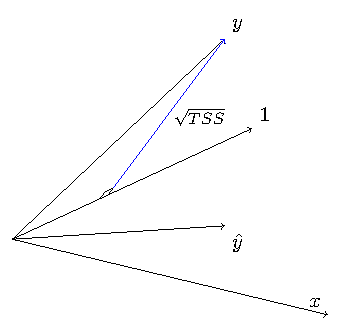
\includegraphics[width=0.4\linewidth]{images/tss_sum_tss.pdf}
\label{fig:tss_tss}}
\hspace{4ex}
\subfigure[]{
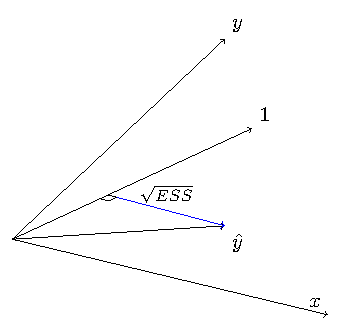
\includegraphics[width=0.4\linewidth]{images/tss_sum_ess.pdf}
\label{fig:tss_ess}}
\caption{\subref{fig:tss_tss}: Total sum of squares; \subref{fig:tss_ess}: Explained sum of squares.}
\end{center}
\end{figure}

The final step is to put everything together.
Note that since $y - \hat y$ is perpendicular to $Lin(x, \mathbf{1})$ it is also perpendicular to $\hat y - \bar y$ and $\mathbf{1}$ as these vectoros are in $Lin(x, \mathbf{1})$.
Then, applying the theorem of three perpendiculars we conclude that the foot of vector $y - \bar y$ is the same point as the foot of the vector $\hat y - \bar y$.
Thus, we obtain a right angle triangle and can apply the Pythagorean theorem for the catheti $\sqrt{RSS}$ and $\sqrt{ESS}$ and the
hypotenuse $\sqrt{TSS}$:
\[
(\sqrt{RSS})^2 + (\sqrt{ESS})^2 = (\sqrt{TSS})^2
\]

\begin{figure}[h!]
\center{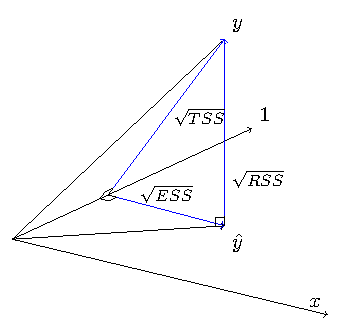
\includegraphics{images/tss_sum_final.pdf}}
\caption{$(\sqrt{RSS})^2 + (\sqrt{ESS})^2 = (\sqrt{TSS})^2$}
\label{fig:tss_final}
\end{figure}

\end{proof}

\subsection{Determination coefficient}

\marginnote{
\begin{align*}
\sCorr^2(y,\hat y) &= \left(\frac{\sCov(y, \hat y)}{\sqrt{\sVar(y)\sVar(\hat y)}}\right)^2 \\
&= \frac{\sCov(y, \hat y) \sCov(y, \hat y)}{\sVar(y)\sVar(\hat y)} \\
&= \frac{\sCov(\hat y + e, \hat y) \sCov(\hat y + e, \hat y)}{\sVar(y)\sVar(\hat y)} \\
&= \frac{(\sCov(\hat y, \hat y) + \sCov(e, \hat y))(\sCov(\hat y, \hat y) + \sCov(e, \hat y))}{\sVar(y)\sVar(\hat y)} \\
&= \frac{\sVar(\hat y) \sVar(\hat y)}{\sVar(y)\sVar(\hat y)} \\
&= \frac{\sVar(\hat y)}{\sVar(y)} \\
&= \frac{ESS}{TSS} \\
&= R^2
\end{align*}
}

\begin{theorem}
A linear regression model with $n$ observations and $k$ explanatory variables including a constant unit vector
\[
y = X \beta + \varepsilon
\]
has the following property
\[
R^2 = \sCorr^2(y, \hat y)
\]
\end{theorem}

\begin{proof}
Proving this theorem geometrically means showing that the determination coefficient can be interpreted as some squared angle
which happens to be eqaul to the squared angle betwen $y$ and $\hat y$.

Consider Figure~\ref{fig:tss_final} from the previous proof.
It was shown there that the vectors $y - \bar y$, $y - \hat y$ and $\hat y - \bar y$ form a right triangle.
Having defined the determination coefficient as
\[
R^2 = \frac{ESS}{TSS}
\]
we conclude that its geometric interpretaion is
\[
\sqrt{R^2} = \frac{\sqrt{ESS}}{\sqrt{TSS}} = \cos \varphi
\]
as shown in Figure~\ref{fig:r_sq_angle}.

\begin{figure}
  \center{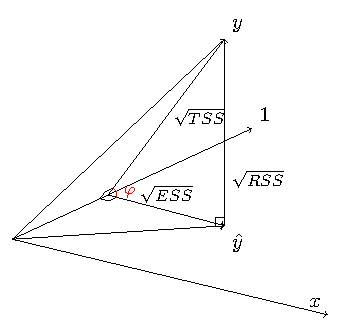
\includegraphics{images/r_sq_ss.pdf}}
  \caption{Determination coefficient as squared $\cos \varphi$}
  \label{fig:r_sq_angle}
\end{figure}

Recall that the sample correlation coefficient two vectors was defined earlier as the angle between these two vectors.
Thus, we conclude that $\sCorr(y, \hat y)$ is the angle between $y$ and $\hat y$ which is also eqaul to $\cos \varphi$.
Finally, squaring both sides, we obtain
\[
R^2 = \sCorr^2(y, \hat y)
\]
\end{proof}

\subsection{Regression line and point of averages}

\marginnote{
If the regression contains the intercept, the following equation holds:
\begin{align*}
\hat y  &= X \hat \beta \\
&= X (X^T X)^{-1} X^T y \\
&= X (X^T X)^{-1} X^T X \beta + X (X^T X)^{-1} X^T \varepsilon
\end{align*}
Premultiplying both sides by $X^T$, we obtain:
\begin{align*}
X^T \hat y &=  X^T X (X^T X)^{-1} X^T X \beta \\
&+ X^T X (X^T X)^{-1} X^T \varepsilon \\
&= X^T X \beta + X^T \varepsilon
\end{align*}
This is a system of equations. The first row of $X^T$ is $\mathbf{1}$ vector, so we can write out the first equation:
\[
\sum_{i=1}^n \hat y_i = \sum_{i=1}^{n} \sum_{j=1}^{k} x_{ij} \beta_{j}
\]
From the first equation in the system
\[
X^T \hat y = X^T y
\]
we obtain
\[
\sum_{i=1}^{n} \hat y_i = \sum_{i=1}^{n} y
\]
And this finishes the proof:
\[
\frac{1}{n} \sum_{i=1}^{n} y = \frac{1}{n} \sum_{i=1}^{n} \sum_{j=1}^{k} x_{ij} \beta_{j}
\]
}

\begin{theorem}
In a linear regression model with one explanatory variable and constant term
\[
y = \beta_1 + \beta_2 x + \varepsilon
\]
the point of averages lies on the estimated regression line.
\end{theorem}

\begin{proof}
For the geometrical proof it suffices to show that $\hat y$ is a linear combination of the regressors, which is true by construction,
and that $\frac{1}{n} \sum_{i=1}^{n} \hat y_i = \frac{1}{n} \sum_{i=1}^{n} y$. In order for the pictures to be more clear the proof will be presented for the case of two regressors.

The first step is regressing $y$ on $Lin(\mathbf{1}, x)$. As shown in Figure~\ref{fig:averages_lin}, we obtain $\hat y$ as a linear combination of $\mathbf{1}$ and $x$.
The next step is to regress both $y$ and $\hat y$ on $\mathbf{1}$ which results in $\bar y$ and $\bar \hat y$ correspondingly.
By the theorem of three perpendiculars, $\bar y = \bar \hat y$ which is shown in Figure~\ref{fig:averages_bars}.

\begin{figure}[ht!]
\begin{center}
\subfigure[]{
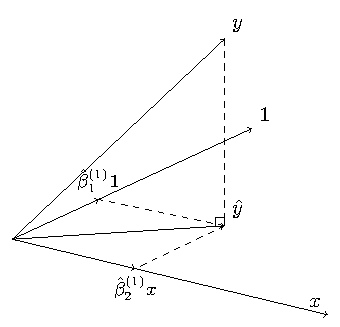
\includegraphics[width=0.4\linewidth]{images/averages_1.pdf}
\label{fig:averages_lin} }
\hspace{4ex}
\subfigure[]{
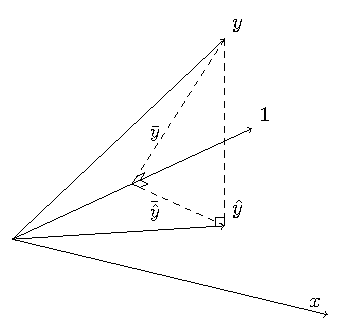
\includegraphics[width=0.4\linewidth]{images/averages_2.pdf}
\label{fig:averages_bars}}
\caption{\subref{fig:averages_lin}: Regression of $y$ on $Lin(\mathbb{1},x)$; \subref{fig:averages_bars}: Regression of $y$ and $\hat y$ on $\mathbb{1}$.}
\end{center}
\end{figure}



\end{proof}

\subsection{Frisch–Waugh–Lovell theorem}

\marginnote{From regresison~\ref{eq:fwl_2} we get the following estimator:
\begin{align*}
\hat\beta_2 &= ((M_1 X_2)^T M_1 X_2)^{-1}(M_1 X_2)^T M_1 y \\
&= (X_2^T M_1^T M_1 X_2)^{-1}  X_2^T M_1^T M_1 y \\
&= (X_2^T M_1 X_2)^{-1}  X_2^T M_1 y
\end{align*}
As for regresison~\ref{eq:fwl_1}, let us note that due to $y = \hat y + \hat u$ $y$ can be decomposed as follows:
\[
y = Py + My = X_1 \hat \beta_1 + X_2 \hat \beta_2 + My
\]
Premultiplying both sides by $X_2^T M_1$, we obtain:
\begin{align*}
X_2^T M_1 y &= X_2^T M_1 X_1 \hat\beta_1 + X_2^T M_1 X_2 \hat\beta_2 + X_2^T M_1 M y \\
&=  X_2^T M_1 X_2 \hat\beta_2 + X_2^T M_1 M y \\
&= X_2^T M_1 X_2 \hat\beta_2
\end{align*}
On the last step we used the fact that
\begin{align*}
(X_2^T M_1 M y)^T = y^T M^T M_1^T X_2 \\
= y^T M M_1 X_2 = y^T M X_2 = 0^T
\end{align*}
Assuming $X_2^T M_1 X_2$ is invertible, we get the same estimator
\[
\hat\beta_2 = (X_2^T M_1 X_2)^{-1}  X_2^T M_1 y
\]
}

\begin{theorem}
Consider regression
\begin{equation} \label{eq:fwl_1}
y = X_1 \beta_1 + X_2 \beta_2 + u
\end{equation}
where $X_{n \times k} = [X_1 X_2]$, i.e. $X_1$ consists of first $k_1$ columns of $X$ and $X_2$ consists of remaining $k_2$ columns of $X$,
$\beta_1$ and $\beta_2$ are comfortable, i.e. $k_1 \times 1$ and $k_2 \times 1$ vectors.
Consider another regresison
\begin{equation}  \label{eq:fwl_2}
M_1 y = M_1 X_2 \beta_2 + M_1 u
\end{equation}
where $M_1 = I - P_1$ projects onto the orthogonal complement of the column space of $X_1$ and $P_1 = X_1(X_1^TX_1)^{-1}X_1^T$ is the projection onto the column space of $X_1$.
Then the estimate of $\beta_2$ from regression~\ref{eq:fwl_1} will be the same as the estimate from regression~\ref{eq:fwl_2}.
\end{theorem}

\begin{proof}
Geometrical proof will be presented for the following model:
\begin{equation} \label{eq:fwl_proof}
y_i = \beta_1 x_i + \beta_2 z_i + u_i
\end{equation}

We start with regression `all-at-once' and will distinct its coefficients with index $(1)$. The only step in obtaining $\beta_1^{(1)}$ is regressing $y$ on $Lin(x,z)$ and then expanding $\hat y$ as a linear combination of basis vectors $x$ and $z$,
which is shown in Figure~\ref{fig:fwl_1_regression_3d}. Figure~\ref{fig:fwl_1_regression_lin} depicts $Lin(x, z)$.

\begin{figure}[ht!]
\begin{center}
\subfigure[]{
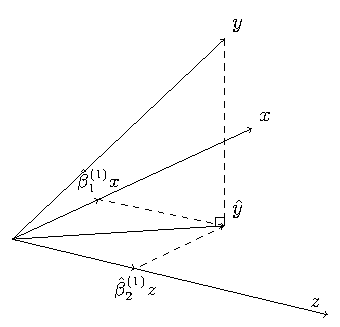
\includegraphics[width=0.4\linewidth]{images/fwl_1_regression.pdf}
%\caption{Regression of $y$ on $Lin(x,z)$} %% подпись к рисунку
\label{fig:fwl_1_regression_3d} }
\hspace{4ex}
\subfigure[]{
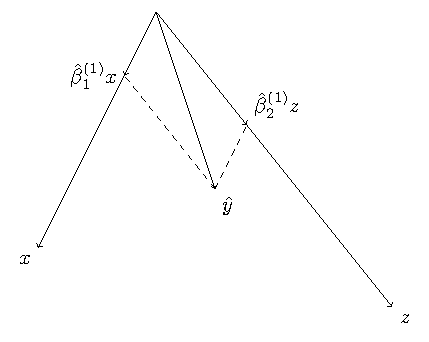
\includegraphics[width=0.4\linewidth]{images/fwl_1_regression_lin.pdf}
%\caption{$Lin(x, z)$}
\label{fig:fwl_1_regression_lin}}
\caption{\subref{fig:fwl_1_regression_3d}: Regression of $y$ on $Lin(x,z)$; \subref{fig:fwl_1_regression_lin}: $Lin(x, z)$.}
\end{center}
\end{figure}

As for the model~\ref{eq:fwl_2}, where several regressions are performed consecutively, we start with regressing $y$ on $z$, resulting in $\tilde{y}$, which we will refer to as ``cleansed'' $y$.

\begin{equation}\label{eq:fwl_2_y_clean}
\begin{aligned}
y &= \alpha z + \varepsilon \\
\hat\alpha &= \frac{y^T z}{z^T z} \\
\tilde{y} &= \hat\varepsilon = y - \frac{y^T z}{z^T z}z
\end{aligned}
\end{equation}

Following that, $x$ is regressed on $z$, resulting in $\tilde{x}$ — ``cleansed'' $x$.

\begin{equation}\label{eq:fwl_2_x_clean}
\begin{aligned}
x &= \gamma z + \nu \\
\hat\gamma &= \frac{x^T z}{z^T z} \\
\tilde{x} &= \hat\nu = x - \frac{x^T z}{z^T z}z
\end{aligned}
\end{equation}

Geometric results of these two steps are presented in~\ref{fig:fwl_2_regression_first}.

Finally, `cleansed' $y$ must be regressed on `cleansed' $x$. However, it cannot be performed immediately as $\tilde{y}$ and $\tilde{x}$ are skew lines.
So at first, we fix this problem by translation and after taht obtain $\hat\beta_1^{(2)}\tilde x$ (see Figure~\ref{fig:fwl_2_regression_trans}).

\begin{figure}[ht!]
\begin{center}
\subfigure[]{
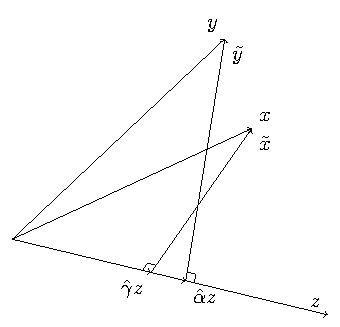
\includegraphics[width=0.4\linewidth]{images/fwl_2_regression.pdf}
%\caption{Regression of $y$ on $Lin(x,z)$} %% подпись к рисунку
\label{fig:fwl_2_regression_first} }
\hspace{4ex}
\subfigure[]{
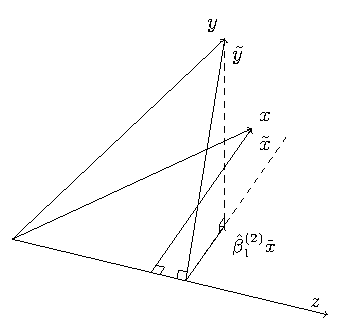
\includegraphics[width=0.4\linewidth]{images/fwl_2_regression_translation.pdf}
%\caption{$Lin(x, z)$}
\label{fig:fwl_2_regression_trans}}
\caption{\subref{fig:fwl_2_regression_first}: Regression of $y$ on $z$ and of $x$ on $z$;
\subref{fig:fwl_2_regression_trans}: Translation of $\tilde{x}$.}
\end{center}
\end{figure}

Now, let us picture all the results in one figure and mark some main points.

\begin{figure}[ht!]
\begin{center}
\subfigure[]{
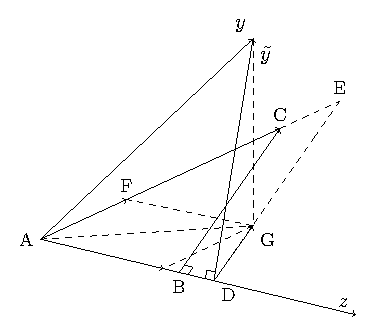
\includegraphics[width=0.4\linewidth]{images/fwl_3_3d.pdf}
%\caption{Regression of $y$ on $Lin(x,z)$} %% подпись к рисунку
\label{fig:fwl_3_3d} }
\hspace{4ex}
\subfigure[]{
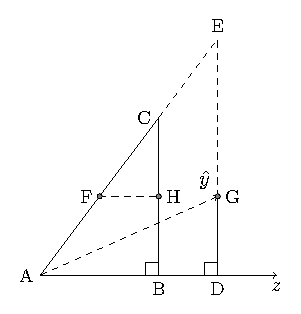
\includegraphics[width=0.4\linewidth]{images/fwl_3_lin.pdf}
%\caption{$Lin(x, z)$}
\label{fig:fwl_3_lin}}
\caption{\subref{fig:fwl_3_3d}: Point A stands for the origin, B — $\hat\gamma z$,
C — $x$, D — $\hat\alpha z$, E — intersection of vector $x$ and line parallel to $\tilde x$,
F — $\hat\beta_1^{(1)} x$, G — $\hat\beta_1^{(2)} \tilde{x}$; \subref{fig:fwl_3_lin}: $Lin(x,z)$.}
\end{center}
\end{figure}

In Figure~\ref{fig:fwl_3_lin} segments AF and BH = DG stand for $\hat\beta_1^{(1)}x$
and $\hat\beta_1^{(2)}\tilde x$ respectively, while segments AC and BC represent $x$ and $\tilde{x}$.
Having two congruent angles, triangles ABC and FHC are simillar.
Then, it follows:
\[
\frac{AF}{AC} = \frac{BH}{BC} \Leftrightarrow \frac{\hat\beta_1^{(1)}x}{x} = \frac{\hat\beta_1^{(2)}\tilde x}{\tilde x} \Leftrightarrow \hat\beta_1^{(1)} = \hat\beta_1^{(2)}
\]
\end{proof}


%\section{Geometric properties of distributions}

\section{Partial correlation}

\subsection{Definition of partial correlation}

\marginnote{
Partial correlation is the measure of degree of dependence between two random
variables while controlling for the effect of other random variables:
\[
\pCorr(X,Y; Z) = \frac{\pCov(X,Y;Z)}{\sqrt{\pVar(X;Z)\pVar(Y;Z)}}
\]
where $\pVar(X;Z) = \Var(X - \alpha Z)$, $\alpha$ is such a constant that $\Cov(X - \alpha Z, Z) = 0$,
and $\pCov(X,Y; Z) = \Cov(X - \alpha Z, Y - \beta Z)$, $\alpha$, $\beta$ are such
constants that $\Cov(X - \alpha Z, Z) = \Cov(Y - \beta Z, Z) = 0$
}

Partial correlation can be defined into two ways.
We will provide both definitions and show their equivalence.

\begin{definition}
Partial correlation between random variables $X$ and $Y$ holding random variable $Z$
fixed is the correlation coefficient between the residuals in regression of $X$ onto
$Z$ and the residuals in regression of $Y$ onto $Z$.
\end{definition}

Firstly, we project random variable $X$ onto $Z$, which yields $\E(X)$.
The residuals in this regression are $X - \E(X)$ — a vector in $Lin^{\perp}(Z)$.
We will call this variable `centered' and label it as $\widetilde X$.
Repeating this step for $Y$ yields `centerd' variable $\tilde Y = Y - \E(Y) \in Lin^{\perp}(Z)$.
The angle between $\widetilde X$ and $\widetilde Y$ ($\varphi$ in Figure~\ref{fig:pcorr_def1})
is the correaletion coefficient between these `centred' random variables and
the partial correlaiton between the original ones.

\begin{figure}
  \centering
  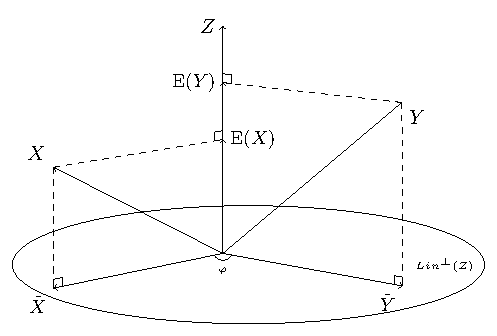
\includegraphics[width=0.55\linewidth]{images/partial_corr.pdf}
  \caption{Partial correlation between $X$ and $Y$ while $Z$ is fixed.}
  \label{fig:pcorr_def1}
\end{figure}

\begin{definition}
Partial correlaiton between random variables $X$ and $Y$ holding random variable $Z$
fixed is the geometric mean between the coefficient $\hat \beta_{XY}$ in regression
\[
\hat X = \hat \beta_{XY} Y + \hat \beta_{XZ} Z
\]
and the coefficinent $\hat \beta_{YX}$ in regression
\[
\hat Y = \hat \beta_{YX} X + \hat \beta_{YZ} Z
\]
which has the same sign as the coefficients $\hat \beta_{XY}$ and $\hat \beta_{YX}$.
\end{definition}

Following the definition, we need to start with regressing variable $X$ onto
$Y$ and $Z$. Then, the vector we obtained $\hat X$ can be broken up into the sum of
$\hat \beta_{XY} Y$ and $\hat \beta_{XZ} Z$.
Projecting $\hat \beta_{XY} Y$ onto $Lin^{\perp}(Z)$ we results in a vector
$\alpha \widetilde Y$ where $\widetilde Y = Y - \E(Y)$ is the projection of $Y$ onto $Lin^{\perp}(Z)$.

By the properties of similar triangles
\[
\frac{\beta_{XY} Y}{Y} = \frac{\alpha \widetilde Y}{\widetilde Y} \Leftrightarrow \beta_{XY} = \alpha
\]

In the same way we perform a regression of $Y$ onto $X$ and $Z$ and repeat the
same steps as for $X$. Finally, we get the whole picture:

\begin{figure}[ht!]
\begin{center}
\subfigure[]{
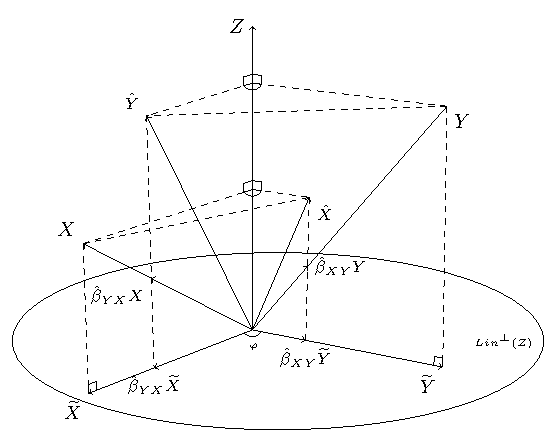
\includegraphics[width=0.55\linewidth]{images/part_corr_2.pdf}
\label{fig:part_corr_alt}}
%\hspace{4ex}
\subfigure[]{
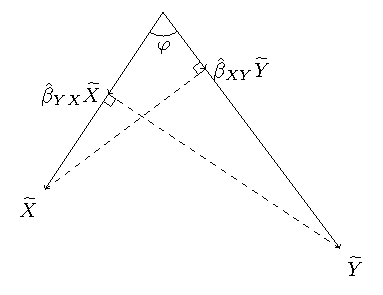
\includegraphics[width=0.35\linewidth]{images/part_corr_2_lin.pdf}
\label{fig:part_corr_alt_lin}}
\caption{\subref{fig:part_corr_alt}: Alternative definition of the partial correlation;
\subref{fig:part_corr_alt_lin}: $Lin^{\perp}(Z)$.}
\end{center}
\end{figure}

Having plotted $Lin^{\perp}(Z)$ now we can express $\cos \varphi$ in terms of $\beta_{XY}$
and $\beta_{YX}$

\begin{equation}\label{eq:part_cor_cos}
\begin{split}
\cos \varphi &= \frac{\vert \beta_{XY} \widetilde Y \vert}{\vert \widetilde X \vert} = \vert \beta_{XY} \vert \\
\cos \varphi &= \frac{\vert \beta_{YX} \widetilde X \vert}{\vert \widetilde Y \vert} = \vert \beta_{YX} \vert \\
\cos^2 \varphi &= \vert \beta_{XY} \beta_{YX} \vert \stackrel{sign(\beta_{XY}) = sign(\beta_{YX})}{=} \beta_{XY} \beta_{YX}
\end{split}
\end{equation}

Recall that the angle $\varphi$ can be interpreted as the partial correlation
between $X$ and $Y$ holding $Z$ fixed, so it follows form equaitions~\eqref{eq:part_cor_cos}

\[
\pCorr^2(X,Y; Z) = \cos^2 \varphi = \beta_{XY} \beta_{YX}
\]

\end{document}
